\section{Modeling Transmission Spectra}

\begin{figure*}[htb]
\begin{center}
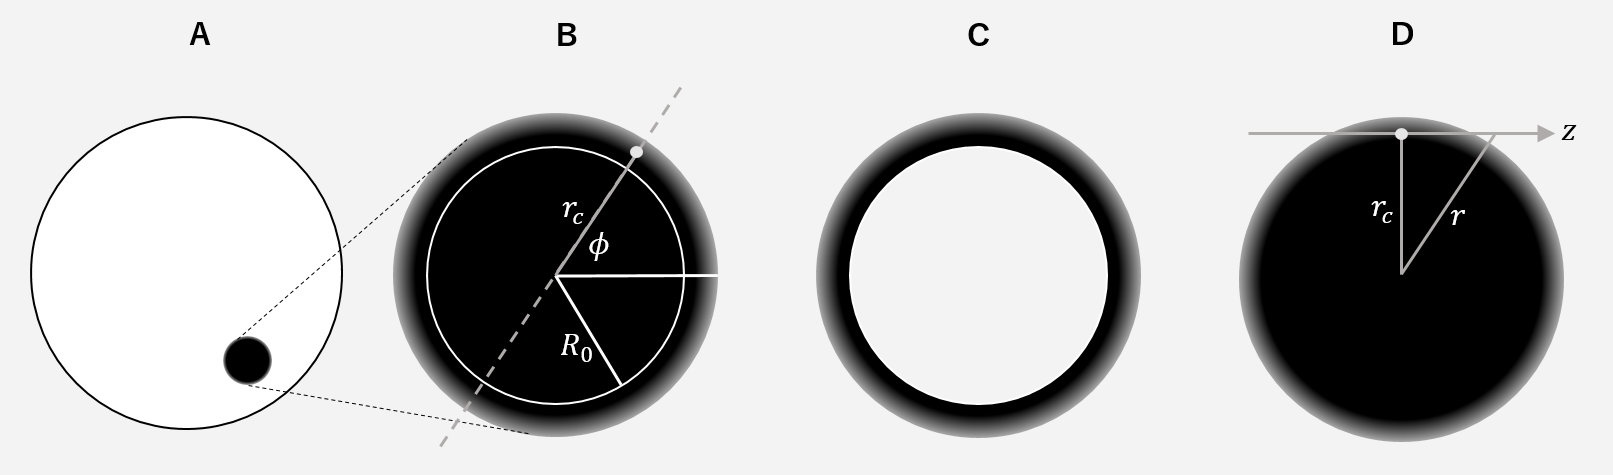
\includegraphics[width=0.85\linewidth]{fig/transmission_chord.PNG}
\caption{Coordinate system for transmission spectroscopy. A: a planet transiting in front of its host star. B: magnified view of the planetary limb. C: the annular shadow region. D: a cut through the planet along the dashed line in panel B. The $z$-direction, along which starlight propagates, is called the chord direction. The right-hand panel corresponds to Fig.~4.13 in \emph{Exoplanet Exploration}. \label{fig:transmission_chord}}
\end{center}
\end{figure*}

Figure~\ref{fig:transmission_chord} illustrates the geometry during transit.
In transmission spectroscopy the quantity of interest is the wavelength dependence of the transmittance through the thin atmospheric layer near the planetary radius. We therefore define a reference radius $R_0$ below which the transmission is sufficiently low (i.e., effectively opaque), and consider only the effective occulted area of the atmospheric annulus above $R_0$, denoted $A(\lambda)$ (hereafter, the \emph{annular shadow}; panel C of Fig.~\ref{fig:transmission_chord}).

For example, if we are interested only in the transit depth, writing the planetary and stellar radii at wavelength $\lambda$ as $R_p(\lambda)$ and $R_\star(\lambda)$, respectively, we have
\begin{align}
\delta(\lambda) = \frac{R_p^2(\lambda)}{R_\star^2(\lambda)}  = \frac{\pi R_0^2 + A(\lambda)}{\pi R_\star^2(\lambda)} ,
\end{align}
so we need only model the annular shadow.\footnote{If ingress/egress is modeled, only a portion of the annulus contributes to the transmission and the geometry is more complicated; we do not consider that here.}

We now derive $A(\lambda)$ for the annular region (Fig.~\ref{fig:transmission_chord}C).
Adopt the coordinates shown in Fig.~\ref{fig:transmission_chord}B/D.
The annular shadow area is
\begin{align}
A &= \int_0^{2 \pi} \int_{R_0}^\infty \!\!\left[ 1 - \mathcal{T}_\lambda(r_c, \phi)\right] r_c \, d r_c \, d\phi \nonumber \\
&= \pi \left( 2 \int_{R_0}^\infty \left[ 1 - \mathcal{T}_\lambda(r_c, \phi)\right] r_c \, d r_c \right),
\end{align}
and the effective wavelength-dependent planetary radius can be written
\begin{align}
    \label{eq:rp_trans}
    R_p(\lambda) = \sqrt{ R_0^2 + 2 \int_{R_0}^\infty \!\!\left[ 1 - \mathcal{T}_\lambda(r_c, \phi)\right] r_c \, d r_c } .
\end{align}
Here $\mathcal{T}_\lambda(r_c,\phi)$ is the chord-direction transmittance at cylindrical radius $r_c$ and wavelength $\lambda$. It is related to the chord optical depth $t$ by
\begin{align}
  \mathcal{T}_\lambda(r_c) = e^{-t}.
\end{align}
For brevity we drop the subscript $\lambda$ below.

Let $z$ be the coordinate along the chord direction. The chord optical depth is
\begin{align}
    t(r_c) = \int_{-\infty}^\infty \kappa(r)\, \rho(r)\, dz
           = 2 \int_{0}^\infty \kappa(r)\, \rho(r)\, dz ,
\end{align}
which we evaluate using a layered-atmosphere model. Denote by $t_n$ the chord optical depth associated with the $n$-th layer. From Fig.~\ref{fig:transmission_coord},
\begin{align}
    t_n &= 2 \sum_k \kappa_k \rho_k \, \Delta z^{(n)}_k .
\end{align}
Here $\Delta z^{(n)}_k$ is the chord-path thickness across the $k$-th layer segment intercepted by the chord tangent to layer $n$. Relating this to the vertical (1D) optical depth of the $k$-th layer, $\Delta \tau_k = \kappa_k \rho_k \Delta r_k$, we obtain
\begin{align}
    t_n &= \sum_k  C_{nk} \, \Delta \tau_k ,\\
    \label{eq:chord_geo_matrix}
    C_{nk} &\equiv \frac{2 \Delta z^{(n)}_k}{\Delta r_k}
    = 2 \,\frac{\sqrt{r_{k-1}^2 - r_{n}^2} - \sqrt{r_{k}^2 - r_{n}^2}}{r_{k-1} - r_{k}} ,
\end{align}
with $r_{N-1}=R_0$. The matrix $C=\{C_{nk}\}$ is a lower-triangular \emph{Chord Geometric Matrix}.

Let $N$ be the total number of layers ($n=0,1,\dots,N-1$).
The radii of the layer boundaries satisfy
\begin{align}
r_{n-1} = r_n + \Delta h_n .
\end{align}
We adopt the boundary convention that the lowest atmospheric layer is $n=N-1$ and define $R_0=r_{N-1}$ as the reference radius from the planet center to the lower boundary of the lowest layer; below $r_{N-1}$ no light is transmitted. Thus
\begin{align}
    r_{n} =
\left\{
\begin{array}{ll}
\displaystyle R_0 + \sum_{j=n+1}^{N-1} \Delta h_j , & n < N-1, \\[6pt]
R_0 , & n = N-1 .
\end{array}
\right.
\end{align}
The upper boundary of the top layer ($n=0$) defines the top of atmosphere (TOA) radius $r_{\mathrm{top}}$.

Because the layers are specified by $(T_n,P_n)$, we convert to geometric thickness using the local scale height,
\begin{align}
\Delta h_n &=  H_n \frac{\Delta P_n}{P_n} ,\\
\label{eq:H_each}
 H_n &= \frac{k_B T_n}{g_n \mu_n m_H} .
\end{align}
The local gravitational acceleration is
\begin{align}
g_n = \frac{G \, (M_p + \Delta M_n)}{r_n^2} ,
\end{align}
where $\Delta M_n = \sum_{j=N-1}^{n} \Delta m_j$ is the cumulative atmospheric mass above $r_n$. In practice $\Delta M_n \ll M_p$ and can usually be neglected.

Numerically, one proceeds upward from the bottom: for $n = N-1, N-2, \dots, 0$ solve for $\Delta h_n$ and $r_n$. The boundary conditions are $r_N = R_0$ and $g_N = G M_p / r_N^2$. We also set $h_0=0$ so that the opacity of the very topmost layer is excluded. While iterating, compute $C_{nk}$ for each layer $n$ and $k=n,\dots, N-1$; this yields the lower-triangular Chord Geometric Matrix.\footnote{Equivalently, after all $r_n$ have been computed, one may evaluate $C_{nk}$ in a single pass using Eq.~(\ref{eq:chord_geo_matrix}).}

\begin{figure*}[htb]
\begin{center}
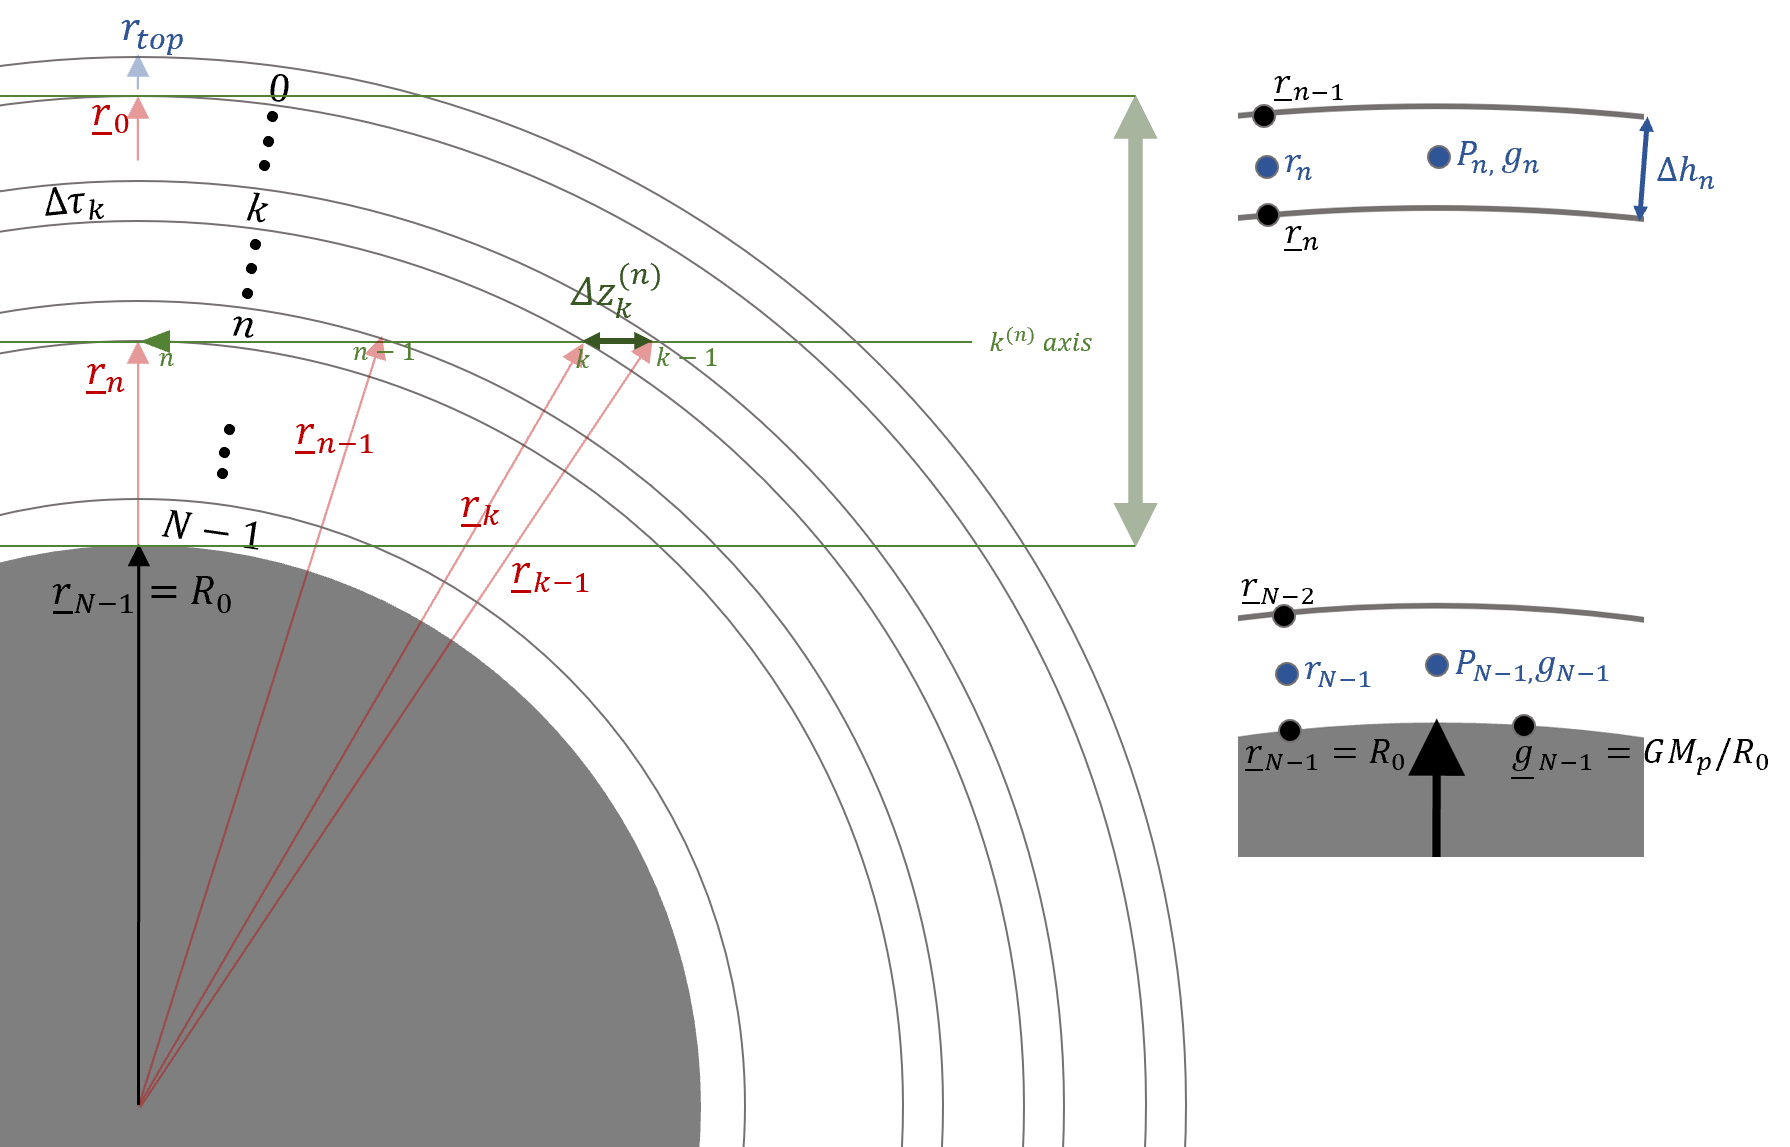
\includegraphics[width=1.0\linewidth]{fig/transmission_coord.PNG}
\caption{Directions of optical-depth integration in the layered model. \label{fig:transmission_coord}}
\end{center}
\end{figure*}
